\documentclass{article}

% Símbolos
\usepackage{recycle}
\usepackage{amsfonts}

% Figuras
\usepackage{graphicx}

% Gráficas
\usepackage{tikz}

% Estilo Tikz
\tikzstyle{edge}=[shorten <=2pt, shorten >=2pt,
                  >=stealth, line width=1.1pt]
\tikzstyle{vertex}=[circle, fill=white, draw,
                    minimum size=5pt,
                    inner sep=0pt, outer sep=0pt]

% Márgenes
\addtolength{\voffset}{-1cm}
\addtolength{\hoffset}{-1.5cm}
\addtolength{\textwidth}{3cm}
\addtolength{\textheight}{2cm}

% Encabezados y Pies de Página
\usepackage{fancyhdr}
% Información del Encabezado
\lhead{Teor\'ia de Gr\'aficas II 2021-2 \\
       Tarea 1}
\rhead{Profesor: C\'esar Hern\'andez Cruz \\
       Ayudante: Daniel Garc\'ia Argueta}
% Información del Pie de Página
\rfoot{\recycle}
\cfoot{\vspace{-0.8cm}?`Realmente necesitas imprimir esta hoja?}
\lfoot{\recycle}
\pagenumbering{gobble}
\footskip = 50pt
% Línea del encabezado
\renewcommand\headrulewidth{1.5pt}
%%%%%%%%%%%%%%%%%%%%%%%%%%%%%%%%%%%%%%%%%%%%%%%%%%%%%%%%%%%%%
%%%%%%%%%%%%%%%%%%%%%%%%%%%%%%%%%%%%%%%%%%%%%%%%%%%%%%%%%%%%%
%%%%%%%%%%          Gráfica en encabezado          %%%%%%%%%%
%%%%%%%%%%%%%%%%%%%%%%%%%%%%%%%%%%%%%%%%%%%%%%%%%%%%%%%%%%%%%
%%%%%%%%%%%%%%%%%%%%%%%%%%%%%%%%%%%%%%%%%%%%%%%%%%%%%%%%%%%%%
\makeatletter
\def\headrule{{\if@fancyplain\let\headrulewidth\plainheadrulewidth\fi
\hrule\@height\headrulewidth\@width\headwidth
\vspace{0.1cm}
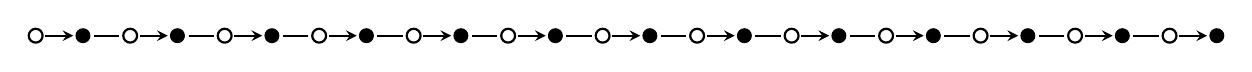
\begin{tikzpicture}
  \begin{scope}[scale=0.6]
   \foreach \x in {0,2,...,24} {
      \node [circle,draw,thick,inner sep=0,minimum size=5pt] (\x) at (\x,0){};
   }
   \foreach \x in {1,3,...,25} {
      \node [circle,draw,fill=black,inner sep=0,minimum size=5pt] (\x) at (\x,0){};
   }
   \foreach \x/\y in {0,2,...,24} {
     \pgfmathsetmacro\result{\x + 1}
     \draw [->,>=stealth,shorten <=3.5pt, shorten >=3.5pt,line width=0.7pt] (\x,0) to (\result,0);
   }
   \foreach \x/\y in {1,3,...,23} {
     \pgfmathsetmacro\result{\x + 1}
     \draw [>=stealth,shorten <=4pt, shorten >=4pt,line width=0.7pt] (\x,0) to (\result,0);
   }
   % \node [inner sep=0,minimum size=5pt] (25.5) at (25.5,-0.05){$\cdots$};
  \end{scope}
\end{tikzpicture}
\vskip-\headrulewidth
\vskip-1.5pt}}
\makeatother
%%%%%%%%%%%%%%%%%%%%%%%%%%%%%%%%%%%%%%%%%%%%%%%%%%%%%%%%%%%%%
%%%%%%%%%%%%%%%%%%%%%%%%%%%%%%%%%%%%%%%%%%%%%%%%%%%%%%%%%%%%%
%%%%%%%%%%%%%%%%%%%%%%%%%%%%%%%%%%%%%%%%%%%%%%%%%%%%%%%%%%%%%
%%%%%%%%%%%%%%%%%%%%%%%%%%%%%%%%%%%%%%%%%%%%%%%%%%%%%%%%%%%%%
%%%%%%%%%%%%%%%%%%%%%%%%%%%%%%%%%%%%%%%%%%%%%%%%%%%%%%%%%%%%%

% Estilo
\pagestyle{fancyplain}

% Macros
\newcommand{\set}[1]{\left\{ #1 \right\}}


\begin{document}

\begin{enumerate}
  \item \textbf{Demuestre que si $D$ es una digr\'afica, entonces su
    condensaci\'on $D^\ast$ es ac\'iclica.}

    Por contradicción, suponga que $D$ es una digráfica, $D^\ast$ su condensación y $C=(C_0,\dots,C_{n-1},C_0)$ un ciclo en ella.. Sea $i\in[n-1]$ y consideremos las componentes $C_i,C_{i+1 mod n}$, ya que $D^\ast$ no tiene lazos, estas son componentes fuertes distintas.

    Veamos que como $(C_i, C_{i+1 modn})\in A(D^\ast)$, por definición de la condensación aseguramos que existe $v_i\in C_i, w_i\in C_{i+1 modn}$ tales que $(v_i,w_i)\in A(D)$. Luego, para cualquier $u\in C_i$, se tiene que por estar en la misma componente fuertemente conexa que $v_i$, entonces existe una $uv_i$-trayectoria ``$P$'', y de forma análoga, para todo $u'\in C_{i+1 modn}$ existe una $w_iu'$-trayectoria ``$P'$''; de ésto se concluye que $\forall i\in[n-1]\forall u\in C_i \forall u'\in C_{i+1 modn}$ existe una $uu'$-trayectoria, a saber $uPv_iw_iP'u'$.

  En síntesis, cualquier vértice de una componente fuertemente conexa en el ciclo $C$ puede alcanzar, en $D$, a todo vértice de la siguiente componente en $C$. Pero, por la naturaleza cíclica de $C$, esto implica que todo vértice de una componente $C_i$, puede alcanzar a todo vértice de otra componente $C_j$, con lo que concluímos que la gráfica inducida por la unión $\cup_{i=1}^nC_i$ es fuertemente conexa, lo que es una contradicción al hecho de que $C$ fuera un ciclo.

  \item \textbf{Demuestre que si $D$ es una digr\'afica ac\'iclica, entonces
    tiene un \'unico n\'ucleo.   Adem\'as, a partir de su demostraci\'on
    obtenga un algoritmo para encontrar un n\'ucleo en una digr\'afica
    ac\'iclica.   ?`Qu\'e complejidad tiene su algoritmo?}

    Por inducción sobre $|V|$. Para $|V|=1$ es claro que se cumple, pues el conjunto $V$ es un núcleo y además es el único.

    Ahora, supongamos que para cualquier digráfica acícilica que cumpla $|V|=k$, tiene un único núcleo. Sea $D$ una digráfica con $|V|=k+1$, luego, por ser acícilica, $D$ tiene una fuente, denotémosla $v$. Veamos que $D'=D-v$ es una digráfica acícilica de $k$ vértices, por lo tanto tiene un único núcleo $N'$.

    Si $N^+(v)\cap N'\neq\emptyset$, entonces $N'$ es un conjunto independiente que absorbe a todo vértice de $D$, por lo tanto es un núcleo de $D$; si por otro lado $N^+(v)\cap N'=\emptyset$, entonces ningún exvecino de $v$ está en $N'$, y por ser una fuente de $D$, no tiene ningún invecino, de aquí se concluye que $N=N'\cup\set{v}$ es un conjunto independiente, y como $N'$ absorbe a todo vértice distinto de $v$, entonces $N$ es un núcleo de $D$.

    Ahora veamos que es único, sea $N_0$ un núcleo cualquiera de $D$, ahora consideremos $N_0-\set{v}$, como $N_0$ absorbe todos los vértices de $D$ y ya que $v$ no tiene invecinos (es decir, ningún vértice es absorbido por él), se tiene que $N_0-\set{v}$ es un núcleo de $D-v$. Pero por hipótesis de inducción éste núcleo era único era único, entonces $N'=N_0-\set{v}$, finalmente, se puede deducir si $v$ es un elemento de $N_0$ usando los mismos argumentos que usamos para construir $N$, y de ésta forma el núcleo de $D$ es único.
%%%%%%%%%%%%%%%%%%%%%%%%%%%%%%%FALTA EL ALGORITMO%%%%%%%%%%%%%%%%%%%%%%%%%%%%%%
  \item \textbf{Demuestre que cualquier digr\'afica con al menos dos n\'ucleos
    contiene un ciclo par.}

    Sea $D$ una digráfica con dos núcleos distintos $N_1,N_2$, definamos $K_1=N_1-N_2$, $K_2=N_2-N_1$, luego, $K=K_1\cup K_2$, notemos que como los núcleos son diferentes, entonces $K\neq\emptyset$. Consideremos $D'=D[K]$.

    Sea $v\in K$, podemos considerar, sin pérdida de la generalidad $v\in K_1$, luego, como $v\notin N_2$ por éste segundo ser un núcleo debe existir $w\in N_2$ tal que $(v,w)\in A_D$, y por ésta adyacencia, se tiene que $w\notin N_1$, por lo tanto $w\in N_2-N_1=K_2\subset K$, es decir $w\in K$.

    De aquí se tiene que $\forall v\in K$ existe $w\in K$ tal que $(v,w)\in A(D)$, es decir $\forall v\in K (d^+_{D'}(v)\geq 1)$, por lo tanto $D'$ tiene un ciclo. Observemos que $K_1$ y $K_2$ son conjuntos independientes, ajenos, y tales que $K=K_1\cup K_2$, entonces ésta es una bipartición de $D'$. Por lo tanto el ciclo debe ser par. Como $D'$ es una subdigráfica inducida, entonces $D$ tiene un ciclo par.

  \item \textbf{Sea $D$ una digr\'afica fuertemente conexa y sea $k > 1$ un entero.
    Demuestre que si todos los ciclos de $D$ tienen longitud congruente a
    $0$ m\'odulo $k$, entonces $V$ admite una partici\'on $V = (V_0, \dots,
    V_{k-1})$ de tal forma que si $(u,v) \in A$, entonces existe $i \in
    \{ 0, \dots, k-1 \}$ tal que $u \in V_i$ y $v \in V_{i+1}$ donde los
    sub\'indices se toman m\'odulo $k$.}

  \item \textbf{Sea $D$ una digr\'afica infinita.  Demuestre que son equivalentes:}
    \begin{enumerate}
      \item \textit{$D$ es n\'ucleo perfecta.}

      \item \textit{Toda subdigr\'afica inducida de $D$ contiene un semin\'ucleo no
        vac\'io.}
    \end{enumerate}
    (Sugerencia: Lema de Zorn.)

  \item \textbf{Para cada entero $k \ge 2$ exhiba una gr\'afica bipartita cuyo
    n\'umero crom\'atico por listas sea al menos $k$.}

  \item \textbf{Demuestre que la digr\'afica de la Figura tiene
    n\'umero crom\'atico por listas igual a $3$.}
    %\label{eje:choose}
    \begin{figure}[ht!]
    \centering
    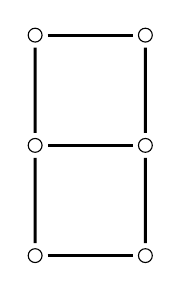
\begin{tikzpicture}
    \begin{scope}[scale=0.7]
      \node (a) at (-1,2)  [vertex]{};
      \node (b) at (-1,0)  [vertex]{};
      \node (c) at (-1,-2) [vertex]{};
      \node (x) at (1,2)   [vertex]{};
      \node (y) at (1,0)   [vertex]{};
      \node (z) at (1,-2)  [vertex]{};

      \foreach \u/\v in {a/b,a/x,y/x,y/b,y/z,c/b,c/z}
        \draw [edge] (\u) to (\v);
    \end{scope}
    \end{tikzpicture}
    \caption{Gr\'afica para el Ejercicio.}
    %\label{fig:choose}
    \end{figure}
\end{enumerate}

\end{document}
